%%%%%%%%%%%%%%%%%%%%%%%%%%%%%%%%%%%%%%%%%%%%%%%%%%%%%%%%%%%%%%%%%%%%%%%%%%%%%%%%
% Template for USENIX papers.
%
% History:
%
% - TEMPLATE for Usenix papers, specifically to meet requirements of
%   USENIX '05. originally a template for producing IEEE-format
%   articles using LaTeX. written by Matthew Ward, CS Department,
%   Worcester Polytechnic Institute. adapted by David Beazley for his
%   excellent SWIG paper in Proceedings, Tcl 96. turned into a
%   smartass generic template by De Clarke, with thanks to both the
%   above pioneers. Use at your own risk. Complaints to /dev/null.
%   Make it two column with no page numbering, default is 10 point.
%
% - Munged by Fred Douglis <douglis@research.att.com> 10/97 to
%   separate the .sty file from the LaTeX source template, so that
%   people can more easily include the .sty file into an existing
%   document. Also changed to more closely follow the style guidelines
%   as represented by the Word sample file.
%
% - Note that since 2010, USENIX does not require endnotes. If you
%   want foot of page notes, don't include the endnotes package in the
%   usepackage command, below.
% - This version uses the latex2e styles, not the very ancient 2.09
%   stuff.
%
% - Updated July 2018: Text block size changed from 6.5" to 7"
%
% - Updated Dec 2018 for ATC'19:
%
%   * Revised text to pass HotCRP's auto-formatting check, with
%     hotcrp.settings.submission_form.body_font_size=10pt, and
%     hotcrp.settings.submission_form.line_height=12pt
%
%   * Switched from \endnote-s to \footnote-s to match Usenix's policy.
%
%   * \section* => \begin{abstract} ... \end{abstract}
%
%   * Make template self-contained in terms of bibtex entires, to allow
%     this file to be compiled. (And changing refs style to 'plain'.)
%
%   * Make template self-contained in terms of figures, to
%     allow this file to be compiled. 
%
%   * Added packages for hyperref, embedding fonts, and improving
%     appearance.
%   
%   * Removed outdated text.
%
%%%%%%%%%%%%%%%%%%%%%%%%%%%%%%%%%%%%%%%%%%%%%%%%%%%%%%%%%%%%%%%%%%%%%%%%%%%%%%%%

\documentclass[letterpaper,twocolumn,10pt]{article}
\usepackage{usenix}

% to be able to draw some self-contained figs
\usepackage{tikz}
\usepackage{amsmath}
\usepackage{amsfonts}
\usepackage[labelfont=bf]{caption}

% inlined bib file
\usepackage{filecontents}

%-------------------------------------------------------------------------------
\begin{filecontents}{\jobname.bib}
%-------------------------------------------------------------------------------
@inproceedings {ULEvsCFS,
  author = {Justinien Bouron and Sebastien Chevalley and Baptiste Lepers and Willy Zwaenepoel and Redha Gouicem and Julia Lawall and Gilles Muller and Julien Sopena},
  title = {The Battle of the Schedulers: {FreeBSD} {ULE} vs. Linux {CFS}},
  booktitle = {2018 USENIX Annual Technical Conference (USENIX ATC 18)},
  year = {2018},
  isbn = {978-1-931971-44-7},
  address = {Boston, MA},
  pages = {85--96},
  url = {https://www.usenix.org/conference/atc18/presentation/bouron},
  publisher = {USENIX Association},
  month = jul
}

@inproceedings{mlfq,
  author = {Corbat{\'o}, Fernando J. and Merwin-Daggett, Marjorie and Daley, Robert C.},
  title = {An experimental time-sharing system},
  year = {1962},
  isbn = {9781450378758},
  publisher = {Association for Computing Machinery},
  address = {New York, NY, USA},
  url = {https://doi.org/10.1145/1460833.1460871},
  doi = {10.1145/1460833.1460871},
  abstract = {It is the purpose of this paper to discuss briefly the need for time-sharing, some of the implementation problems, an experimental timesharing system which has been developed for the contemporary IBM 7090, and finally a scheduling algorithm of one of us (FJC) that illustrates some of the techniques which may be employed to enhance and be analyzed for the performance limits of such a time-sharing system.},
  booktitle = {Proceedings of the May 1-3, 1962, Spring Joint Computer Conference},
  pages = {335–344},
  numpages = {10},
  location = {San Francisco, California},
  series = {AIEE-IRE '62 (Spring)}
}

@inproceedings{DRR,
  author = {Shreedhar, M. and Varghese, George},
  title = {Efficient fair queueing using deficit round robin},
  year = {1995},
  isbn = {0897917111},
  publisher = {Association for Computing Machinery},
  address = {New York, NY, USA},
  url = {https://doi.org/10.1145/217382.217453},
  doi = {10.1145/217382.217453},
  abstract = {Fair queuing is a technique that allows each flow passing through a network device to have a fair share of network resources. Previous schemes for fair queuing that achieved nearly perfect fairness were expensive to implement: specifically, the work required to process a packet in these schemes was O(log(n)), where n is the number of active flows. This is expensive at high speeds. On the other hand, cheaper approximations of fair queuing that have been reported in the literature exhibit unfair behavior. In this paper, we describe a new approximation of fair queuing, that we call Deficit Round Robin. Our scheme achieves nearly perfect fairness in terms of throughput, requires only O(1) work to process a packet, and is simple enough to implement in hardware. Deficit Round Robin is also applicable to other scheduling problems where servicing cannot be broken up into smaller units, and to distributed queues.},
  booktitle = {Proceedings of the Conference on Applications, Technologies, Architectures, and Protocols for Computer Communication},
  pages = {231–242},
  numpages = {12},
  location = {Cambridge, Massachusetts, USA},
  series = {SIGCOMM '95}
}

@misc{sysbench,
  author = {Alexey Kopytov},
  title = {sysbench: Scriptable database and system performance benchmark},
  howpublished = {\url{https://github.com/akopytov/sysbench}},
  note = {GitHub repository}
}
\end{filecontents}

\usetikzlibrary{matrix, positioning, calc, arrows.meta}

%-------------------------------------------------------------------------------
\begin{document}
%-------------------------------------------------------------------------------

%don't want date printed
\date{}

% make title bold and 14 pt font (Latex default is non-bold, 16 pt)
\title{\Large \bf eBPF Scheduler Proposal: A Multi-dimensional Multilevel Feedback Queue Scheduler}

%for single author (just remove % characters)
\author{
{\rm Jeffrey Jiang}\\
Stony Brook University
} % end author

\maketitle

%-------------------------------------------------------------------------------
\section{Motivation}
%-------------------------------------------------------------------------------

Kernel schedulers are responsible for determining how to best utilize the CPU
while remaining performant and flexible under different workloads. The scheduler
must be considerate of the different characteristics of the processes being
scheduled. Two such important properties that a scheduler can take into account
for its decisions are its latency requirements and its ideal time slice length. 
However, existing schedulers such as FreeBSD's ULE scheduler often conflate these 
two properties together. I argue that schedulers should instead treat these two 
properties as orthogonal to each other.

As an example of how schedulers conflate these two properties, consider the ULE
scheduler. The ULE scheduler groups processes into two categories, interactive
processes and batch processes, based on an \emph{interactivity} metric which
is loosely the ratio between the amount of time a thread spends running to
the amount of time a thread spends voluntarily sleeping. ULE always schedule
interactive processes before batch processes because interactive processes
are considered latency sensitive~\cite{ULEvsCFS}. Thus, ULE associates latency
sensitivity with how the proportion that a process spends running. While,
this dichotomy works well, it ignores processes which do not neatly fit into
this dichotomy. For example, a process which spends a lot of time on computations 
but needs to respond quickly to an event would be penalized by ULE because
it would be considered a batch process. The scheduler I am proposing will
solve this issue by treating latency requirements and its ideal time 
slice length orthogonally.

%-------------------------------------------------------------------------------
\section{Proposed Scheduler}
%-------------------------------------------------------------------------------

My proposed scheduler is based on the multilevel feedback queue (MLFQ) 
scheduling~\cite{mlfq} like FreeBSD's ULE except modifications were made 
to treat the latency requirement and the ideal time slice length orthogonally.

\subsection{Data Structure}

My scheduler will use a two-dimensional grid of feedback run queues. 
Figure~\ref{fig:mlfq_grid} shows the structure of the scheduler I am proposing. 
The grid is \(8\times 8\), and each cell is a run queue, represented by a 
circular linked list. The x-axis of the grid represent the time slice length 
assigned processes within queues of that column, and the y-axis represents the 
latency requirement of the process. Together, if a process is in the run 
queue at row \(i\) and column \(j\), then it has the latency requirement assigned 
to row \(i\) and the quantum at column \(j\). The \(8\times 8\) grid was chosen, 
so there is a total of \(64\) queues. This allows a summary of the grid represented 
as a bitset in a \(64\)-bit integer which allows us to use bitwise operations to 
perform operations such as finding the first queue with a process on it.  

\begin{figure}
  \begin{center}
    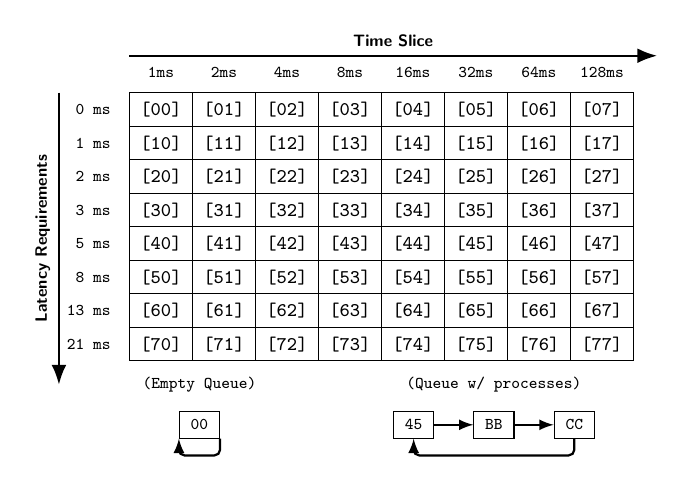
\begin{tikzpicture}[
    scale=0.85, transform shape, % Scales down the entire diagram
    queue node/.style={draw, minimum width=0.6cm, minimum height=0.4cm, anchor=center, font=\scriptsize\ttfamily},
    axis arrow/.style={-{Latex[length=2.5mm]}, thick},
    grid node/.style={draw, minimum width=0.8cm, minimum height=0.4cm, anchor=center, font=\scriptsize\ttfamily}
]
    % Define the grid
    \matrix (mat) [
        matrix of nodes,
        nodes={grid node},
        column sep=-\pgflinewidth,
        row sep=-\pgflinewidth,
        nodes in empty cells=false
    ] {
        |[name=m00]| [00] & |[name=m01]| [01] & |[name=m02]| [02] & |[name=m03]| [03] & |[name=m04]| [04] & |[name=m05]| [05] & |[name=m06]| [06] & |[name=m07]| [07] \\
        |[name=m10]| [10] & |[name=m11]| [11] & |[name=m12]| [12] & |[name=m13]| [13] & |[name=m14]| [14] & |[name=m15]| [15] & |[name=m16]| [16] & |[name=m17]| [17] \\
        |[name=m20]| [20] & |[name=m21]| [21] & |[name=m22]| [22] & |[name=m23]| [23] & |[name=m24]| [24] & |[name=m25]| [25] & |[name=m26]| [26] & |[name=m27]| [27] \\
        |[name=m30]| [30] & |[name=m31]| [31] & |[name=m32]| [32] & |[name=m33]| [33] & |[name=m34]| [34] & |[name=m35]| [35] & |[name=m36]| [36] & |[name=m37]| [37] \\
        |[name=m40]| [40] & |[name=m41]| [41] & |[name=m42]| [42] & |[name=m43]| [43] & |[name=m44]| [44] & |[name=m45]| [45] & |[name=m46]| [46] & |[name=m47]| [47] \\
        |[name=m50]| [50] & |[name=m51]| [51] & |[name=m52]| [52] & |[name=m53]| [53] & |[name=m54]| [54] & |[name=m55]| [55] & |[name=m56]| [56] & |[name=m57]| [57] \\
        |[name=m60]| [60] & |[name=m61]| [61] & |[name=m62]| [62] & |[name=m63]| [63] & |[name=m64]| [64] & |[name=m65]| [65] & |[name=m66]| [66] & |[name=m67]| [67] \\
        |[name=m70]| [70] & |[name=m71]| [71] & |[name=m72]| [72] & |[name=m73]| [73] & |[name=m74]| [74] & |[name=m75]| [75] & |[name=m76]| [76] & |[name=m77]| [77] \\
    };

    % X-axis labels (Quanta) - Moved to top
    \node [above=0.1cm of m00, font=\scriptsize\ttfamily] {1ms};
    \node [above=0.1cm of m01, font=\scriptsize\ttfamily] {2ms};
    \node [above=0.1cm of m02, font=\scriptsize\ttfamily] {4ms};
    \node [above=0.1cm of m03, font=\scriptsize\ttfamily] {8ms};
    \node [above=0.1cm of m04, font=\scriptsize\ttfamily] {16ms};
    \node [above=0.1cm of m05, font=\scriptsize\ttfamily] {32ms};
    \node [above=0.1cm of m06, font=\scriptsize\ttfamily] {64ms};
    \node [above=0.1cm of m07, font=\scriptsize\ttfamily] {128ms};
    
    % Quanta Arrow - Moved to top
    \draw[axis arrow] ([xshift=0.15cm, yshift=0.4cm]mat.north west) -- ([xshift=0.2cm, yshift=0.4cm]mat.north east) node[midway, above, font=\sffamily\bfseries\scriptsize] {Time Slice};

    % Y-axis labels (Latency)
    \node [left=0.15cm of m00, font=\scriptsize\ttfamily] {0 ms};
    \node [left=0.15cm of m10, font=\scriptsize\ttfamily] {1 ms};
    \node [left=0.15cm of m20, font=\scriptsize\ttfamily] {2 ms};
    \node [left=0.15cm of m30, font=\scriptsize\ttfamily] {3 ms};
    \node [left=0.15cm of m40, font=\scriptsize\ttfamily] {5 ms};
    \node [left=0.15cm of m50, font=\scriptsize\ttfamily] {8 ms};
    \node [left=0.15cm of m60, font=\scriptsize\ttfamily] {13 ms};
    \node [left=0.15cm of m70, font=\scriptsize\ttfamily] {21 ms};
    
    % Latency Arrow
    \draw[axis arrow] ([xshift=-0.9cm, yshift=-0.15cm]mat.north west) -- ([xshift=-0.9cm, yshift=-0.2cm]mat.south west) node[midway, above, rotate=90, font=\sffamily\bfseries\scriptsize] {Latency Requirements};

    % Linked List Queue representations with traditional nodes & closed loops
    \begin{scope}[shift={([xshift=1.2cm, yshift=-0.8cm]mat.south west)}] % Shifted down further to accommodate above-labels
        % First list (Empty Queue) - single node routing back to itself
        \node[queue node] (q00) at (0, 0) {00};
        \draw[-latex, thick, rounded corners=2pt] (q00.south east) -- ++(0,-0.25) -| (q00.south west);
        \node[above=0.15cm of q00, font=\scriptsize\ttfamily] {(Empty Queue)};

        % Second list (Queue w/ processes) - positioned horizontally relative to the first
        \node[queue node] (q45a) at (3.2, 0) {45};
        \node[queue node] (qBB) at (4.4, 0) {BB};
        \node[queue node] (qCC) at (5.6, 0) {CC};
        \draw[-latex, thick] (q45a) -- (qBB);
        \draw[-latex, thick] (qBB) -- (qCC);
        \draw[-latex, thick, rounded corners=2pt] (qCC.south) -- ++(0,-0.25) -| (q45a.south);
        % Centered the label above the middle node (qBB)
        \node[above=0.15cm of qBB, font=\scriptsize\ttfamily] {(Queue w/ processes)}; 
    \end{scope}
\end{tikzpicture}
  \end{center}
  \captionsetup{font=scriptsize}
  \vspace{-10pt}
  \caption{\scriptsize\label{fig:mlfq_grid} The scheduler is arranged in a 
  two-dimensional grid. Each cell of the grid is a circular feedback run queue.
  The queue at row 0 and column 0 is empty while the queue at row 4 and column 
  5 contains two processes: \texttt{AA} and \texttt{BB}. Times are subject
  to change.}
\end{figure}

\subsection{Scheduling Policy}

Similar to MLFQ, the scheduler will adaptively move processes between different
queues with the goal to find the ideal queue which best suits the process'
behavior. Because of the grid structure, this involves determining the time
slice length and the latency requirement of the process dynamically. 

\begin{itemize}
  \item \textbf{Time Slice Length:} Move the process up a tier if a process
                                    completes its allotted time slice. Move down
                                    a tier if a process yields before half of
                                    its allotted time slice.
  \item \textbf{Latency Requirement:} Latency requirement is determined via
                                      user-provided hint as well as inspecting
                                      the wait queue that the process awoke from.
                                      For example, a process from a futex wait
                                      queue has a higher latency requirement than
                                      a process waking up due to a network packet.
\end{itemize}

When a process is ready to be scheduled, the scheduler computes the correct
run queue in the grid to place this process within. At this point in time,
the scheduler will preempt the currently running process if the remaining time
slice exceeds the newly awoken process' latency requirement. Otherwise, the
process is simply placed at the tail of the run queue.

When a process completes its time slice, the process is preempted and placed
back into the run queue with a latency requirement penalty to allow another
process to be scheduled. To select the next process to run, the scheduler
will find the first non-empty run queue that first has the lowest latency 
requirement, then the lowest time slice. From this run queue, the scheduler
will schedule the process at the head of the run queue. Currently, this design 
permits starvation. This, however, can be fixed by performing a deficit round 
robin instead when selecting the run queue~\cite{DRR}. 



%-------------------------------------------------------------------------------
\section{Evaluation Plan}
\label{sec:evaluation}
%-------------------------------------------------------------------------------

Evaluation will be performed using a mix of synthetic and real-world benchmarks
on a bare-metal laptop with an Intel Core i7-6700HQ running Linux Mint. This
CPU has a total of 4 cores with 2 threads per core from hyper-threading.

I will be comparing my scheduler against the EEVDF scheduler and potentially the
ULE scheduler implemented in eBPF if time permits. First, I will determine the
cost of the operations involved in my scheduler and compare it with the other
schedulers. I will consider the average and tail latency here. The goal is to 
demonstrate that my scheduler algorithm is feasible for real-world use. 

Next, I will evaluate how well my scheduler performs compared to the baseline.
I will use hackbench which is a traditional benchmark and stress test for
the Linux schedulers and Schbench which provides latency distribution
statistics. I will also construct synthetic benchmarks which represent
processes which are compute-heavy and also latency-sensitive and processes
which sleep often but are latency-insensitive. Based on my hypothesis,
I would expect the baseline schedulers to schedule theses processes poorly, and
I would like to examine if my scheduler performs better. For this, I will examine
how these processes interfere with batch and interactive processes. 

%-------------------------------------------------------------------------------
\section{Expected Outcomes}
%-------------------------------------------------------------------------------

I would expect that my scheduler performs performs better than the baseline
schedulers on some benchmarks, but not all. Existing schedulers have been
highly optimized and the eBPF overhead for my scheduler may be significant
due to the expected low cost of scheduling. However, as laid out currently,
my scheduling algorithm should have an algorithmic complexity of
\(\mathcal{O}(1)\) compared to the \(\mathcal{O}(\log n)\) complexity of
EEVDF.\@ I do expect that my scheduler outperforms EEVDF and ULE when it
comes to the non-traditional processes described in Section~\ref{sec:evaluation}.

\section{Expected Challenges}

I expect implementation of the scheduler to be simple due to its simple data
structure and algorithms involved. However, the main challenge that I believe
I will run into is tuning the parameters of the scheduler. The current design
allows a lot of potential adjustments such as determining the how the latency
requirement and time slice length scales between tiers. I believe this tuning
will be the most crucial in obtaining optimal performance. This will require
a further experimentation after the implementation which may be the most
time-consuming part.

%-------------------------------------------------------------------------------
\bibliographystyle{plain}
\bibliography{\jobname}

%%%%%%%%%%%%%%%%%%%%%%%%%%%%%%%%%%%%%%%%%%%%%%%%%%%%%%%%%%%%%%%%%%%%%%%%%%%%%%%%
\end{document}
%%%%%%%%%%%%%%%%%%%%%%%%%%%%%%%%%%%%%%%%%%%%%%%%%%%%%%%%%%%%%%%%%%%%%%%%%%%%%%%%

%%  LocalWords:  endnotes includegraphics fread ptr nobj noindent
%%  LocalWords:  pdflatex acks